\modeCorrection

\renewcommand{\thesubsection}{\textcolor{red}{\Roman{section}.\arabic{subsection}}}
\renewcommand{\thesubsubsection}{\textcolor{red}{\Roman{section}.\arabic{subsection}.\alph{subsubsection}}}

\setcounter{section}{0}
\sndEnTeteCoursCinq

\begin{mdframed}[style=titr, leftmargin=60pt, rightmargin=60pt, innertopmargin=7pt, innerbottommargin=7pt, innerrightmargin=8pt, innerleftmargin=8pt]

\begin{center}
\large{\textbf{Chapitre 5 : Spectres d'émission de la lumière}}
\end{center}
\end{mdframed}
Dans le chapitre 4, on a vu que le prisme permettait de disperser la lumière émise par une source. Le résultat obtenu est appelé \textcolor{red}{spectre d'émission} de la source. 

\begin{center}
    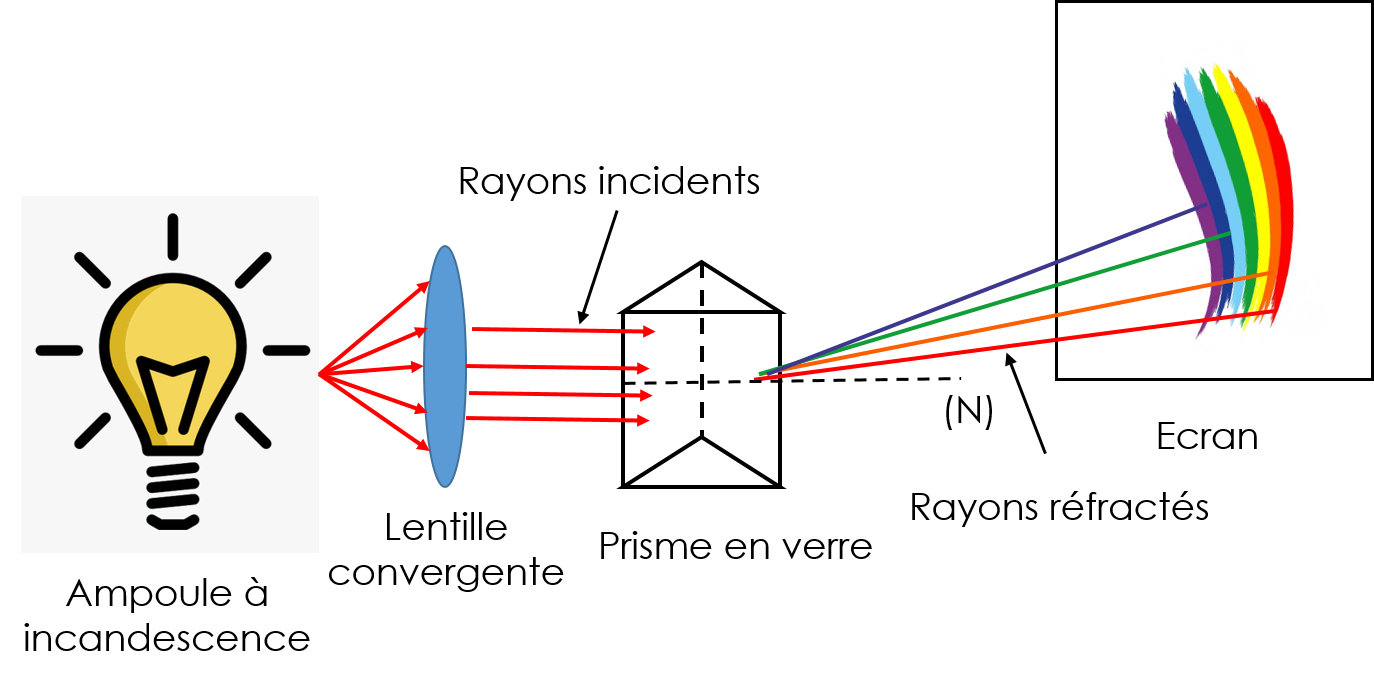
\includegraphics[scale=0.5]{Images/Montage.png}
\end{center}

\begin{tcolorbox}[colback=blue!5!white,colframe=blue!75!black,title=Mots clés du chapitre :]
Spectre continu d'émission, spectre de raies d'émission, longueur d'onde, domaine du visible, température de surface d'un corps 
\end{tcolorbox}


\section{La lumière, une onde électromagnétique}
\begin{minipage}{0.8\textwidth}
Vidéo sur des images des \og Pilliers de la création \fg dans la constellation de l'Aigle par le télescope spatial américano-européen Hubble \url{https://www.youtube.com/watch?v=hZ7zGUFDOsg}.
\end{minipage}
\begin{minipage}{0.2\textwidth}

\includegraphics[scale=0.17]{Images/qrcode_PillierCreation.png}
\end{minipage}
\importantbox{Les couleurs associées à une image prise dans des longueurs d'ondes invisibles aux yeux humains sont issus d'un traitement numérique (artificiel donc) !}
\subsection{Rappels : la vitesse de la lumière dans le vide}
Les ondes électromagnétiques se progagent toutes à la même vitesse dans le vide appelée \textcolor{red}{célérité de la lumière} valant exactement $c =$ 299 792 458~m.s$^{-1}$. 
\begin{tcolorbox}[colback=red!5!white,colframe=red!75!black,title=\textbf{Propriété de la vitesse de la lumière :}]
On retiendra plus facilement la valeur arrondie :
\begin{empheq}[box=\fbox]{equation*}
    c=3,00\times10^8~\text{m$\cdot$s$^{-1}$}
\end{empheq}
\end{tcolorbox}

\subsection{Le domaine visible}
\begin{tcolorbox}
[colback=green!5!white,colframe=green!75!black,title=\textbf{La longueur d'onde et le domaine du visible :}]
Pour différencier les ondes électromagnétiques, on les repère grâce à leur \textcolor{red}{longueur d'onde}, notée $\lambda$, qui s'exprime en nanomètre (ou mètre).\\
Les longeurs d'ondes de la lumière visible pour l'\oe il humain sont comprises entre 400~nm et 800~nm.
\begin{center}
    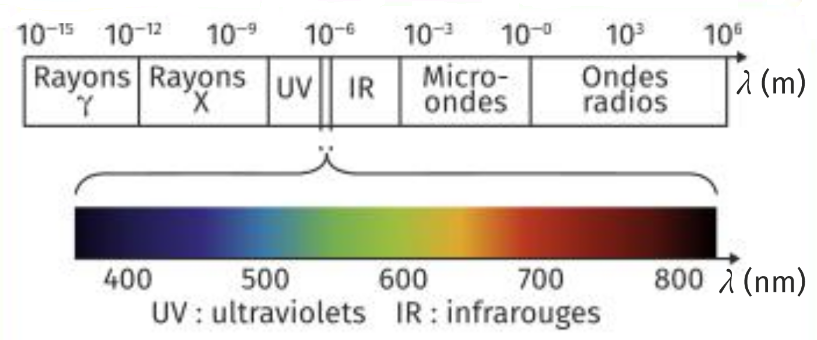
\includegraphics[scale=0.7]{Images/Longueur_onde.PNG}
\end{center}
\end{tcolorbox}

\section{Production de lumière}
\begin{Large}
    \ding{43}
\end{Large}
Voir TP 10 : L'arc-en-ciel
\subsection{Spectre du rayonnement émis par un corps chaud}
\textcolor{blue}{Expérience :} On réalise le spectre de la lumière émise par une ampoule à incandescence. On fait varier la tension imposée à l'ampoule à l'aide d'un potentiomètre. \\
\textit{Observations :} \texteTrouMultiLignes{On voit qu'en augmentant la tension aux bornes de l'ampoule avec le potentiomètre, les couleurs du spectres apparaissent plus vives et le spectre s'enrichit des couleurs bleues et violettes.}{2}

\begin{center}
    
\includegraphics[scale=0.6]{Images/SpectresvsT_commente.png}
\end{center}

\subsection{Activité documentaire : \'{E}tude de l'intensité de l'étoile polaire}
L'étoile polaire a servi aux explorateurs de se repérer depuis des millénaires car elle a la particularité de se situer sur l'axe de rotation de la Terre à tout instant de la nuit.\\
\begin{minipage}{0.45\textwidth}
    \begin{doc}{Une année-lumière}
    L'année lumière est une unité de distance correspondant à la distance parcourue par la lumière pendant 365,25 jours.\\
    L'étoile polaire se trouve à une distance de 450 années-lumière de la Terre. 
    \end{doc}
    \begin{center}
        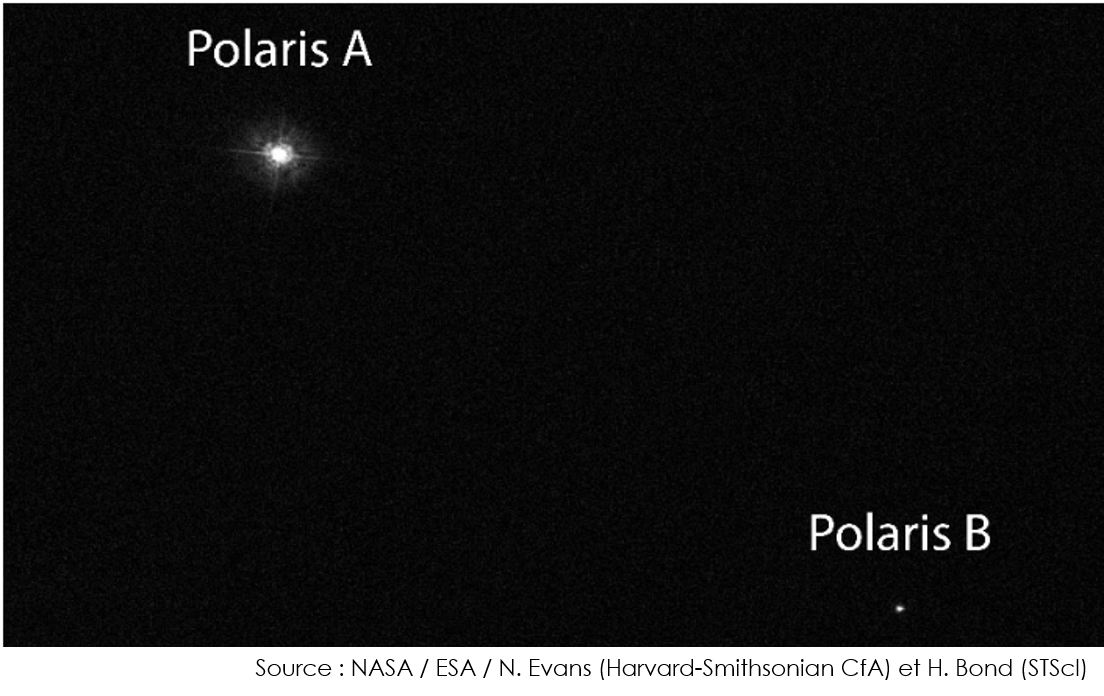
\includegraphics[scale=0.43]{Images/Etoile_polaire.png}
    \end{center}
\end{minipage}
\begin{minipage}{0.54\textwidth}
    \begin{doc}{Classement des étoiles}
     L'étoile Polaire est en réalité un système d'étoiles doubles dont l'étoile la plus massive, \og \textit{Polaris A} \fg~est une céphéide, c’est-à-dire une étoile massive, jeune, très brillante. Les étoiles sont souvent classées suivant un critère : leur température de leur surface. Celle-ci peut s'établir à 3000~K pour les plus froides jusqu'à 30 000~K pour les plus chaudes. Le Kelvin est l'unité de température du système internationale dont la relation avec les degrés Celsius est :
    \begin{equation*}
        \text{T(K) = T($\degreCelsius$)+273,15}
    \end{equation*}
    \vspace{1cm}
    \end{doc}
\end{minipage}
 

%\begin{minipage}{0.6\textwidth}
    \begin{doc}{Longueur d'onde et température de surface d'un corps chaud}
    \begin{center}
        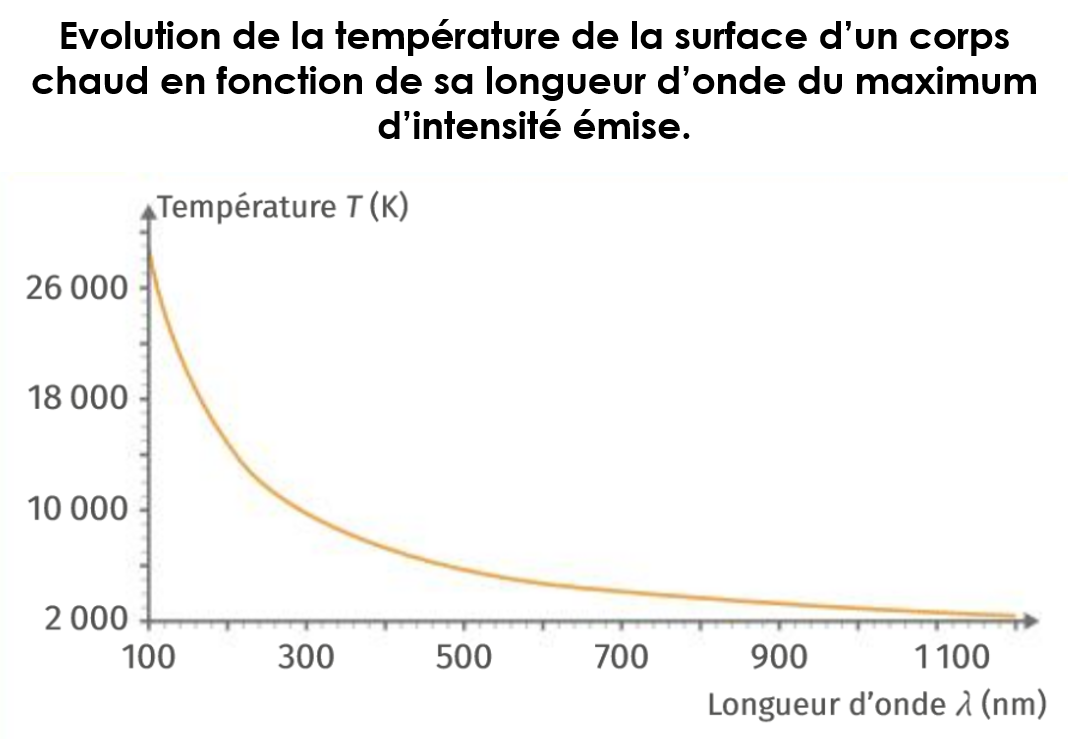
\includegraphics[scale=0.7]{Images/TemperaturevsLongueurdonde.PNG}
    \end{center}
    \end{doc}
%\end{minipage}

\begin{large}
    \textbf{\textcolor{red}{\underline{Travail à réaliser :}}}
\end{large}
\\
\question{Calculer la distance en mètre qui nous sépare de l'étoile Polaire (Document 1).}{On connait $c=3,00\times 10^8$~m.s$^{-1}$ et la formule $d=c\times \Delta t$. Pour une année :
\begin{equation*}
    \Delta t=365,25~\text{jours} = 365,25\times24~\text{heures} = 365,25\times24\times 3600~\text{secondes} =3,1558\times10^7\text{secondes}
\end{equation*}
On en déduit que pour 400 années-lumières :
\begin{equation*}
    d = 400\times 3,00\times10^8\times3,1558\times10^7 = 3,7870\times10^{18}~\text{m}
\end{equation*}}{0}
%\\
\question{Télécharger le fichier \og DonneesEtoilePolaire \fg~dans l'\og Espace documentaire\fg~ de la classe.}{Fait en classe.}{0}
\\
\question{Tracer sur un tableur Excel l'intensité lumineuse émise par \textit{Polaris A} en fonction de la longueur d'onde de la lumière. Mettre un titre sur les axes et sur le graphique.}{\begin{center}
    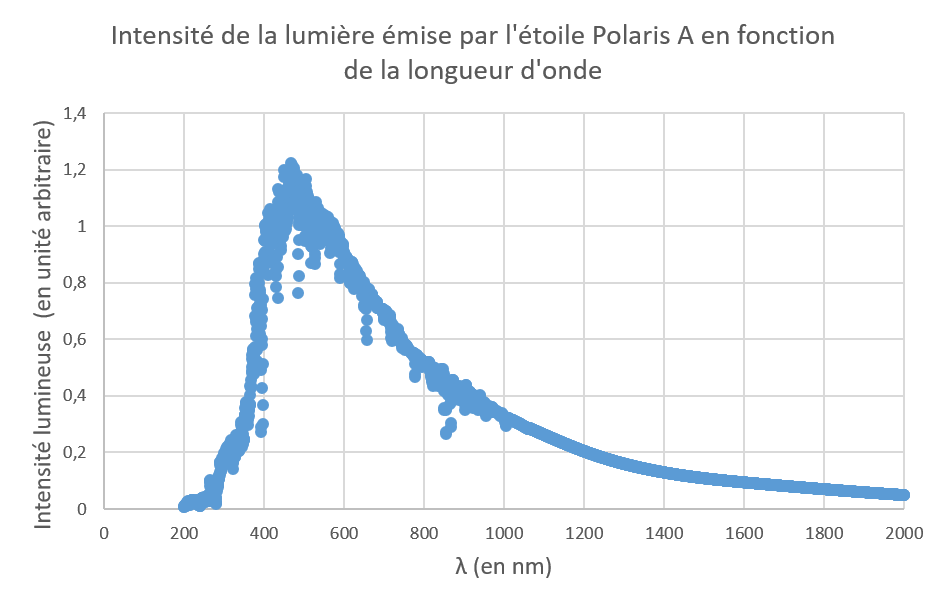
\includegraphics[scale=1]{Images/Intensite_EtoilePolaire.png}
\end{center}}{0}
%\\
\question{Déterminer la longueur d'onde $\lambda_{max}$ au maximum d'intensité de lumière produite par l'étoile Polaire.}{En zoomant autour du maximum d'intensité, on lit : $\lambda_{max}\simeq 468$~nm.}{0}
\\
\question{Cette longueur d'onde est-elle associée au domaine du visible ?}{Oui, $\lambda_{max}\in \left[400~\text{nm},800~\text{nm}\right]$.}{0}
\\
\question{\`{A} l'aide du document 3, déterminer la température à la surface de \textit{Polaris A}.}{\begin{center}
    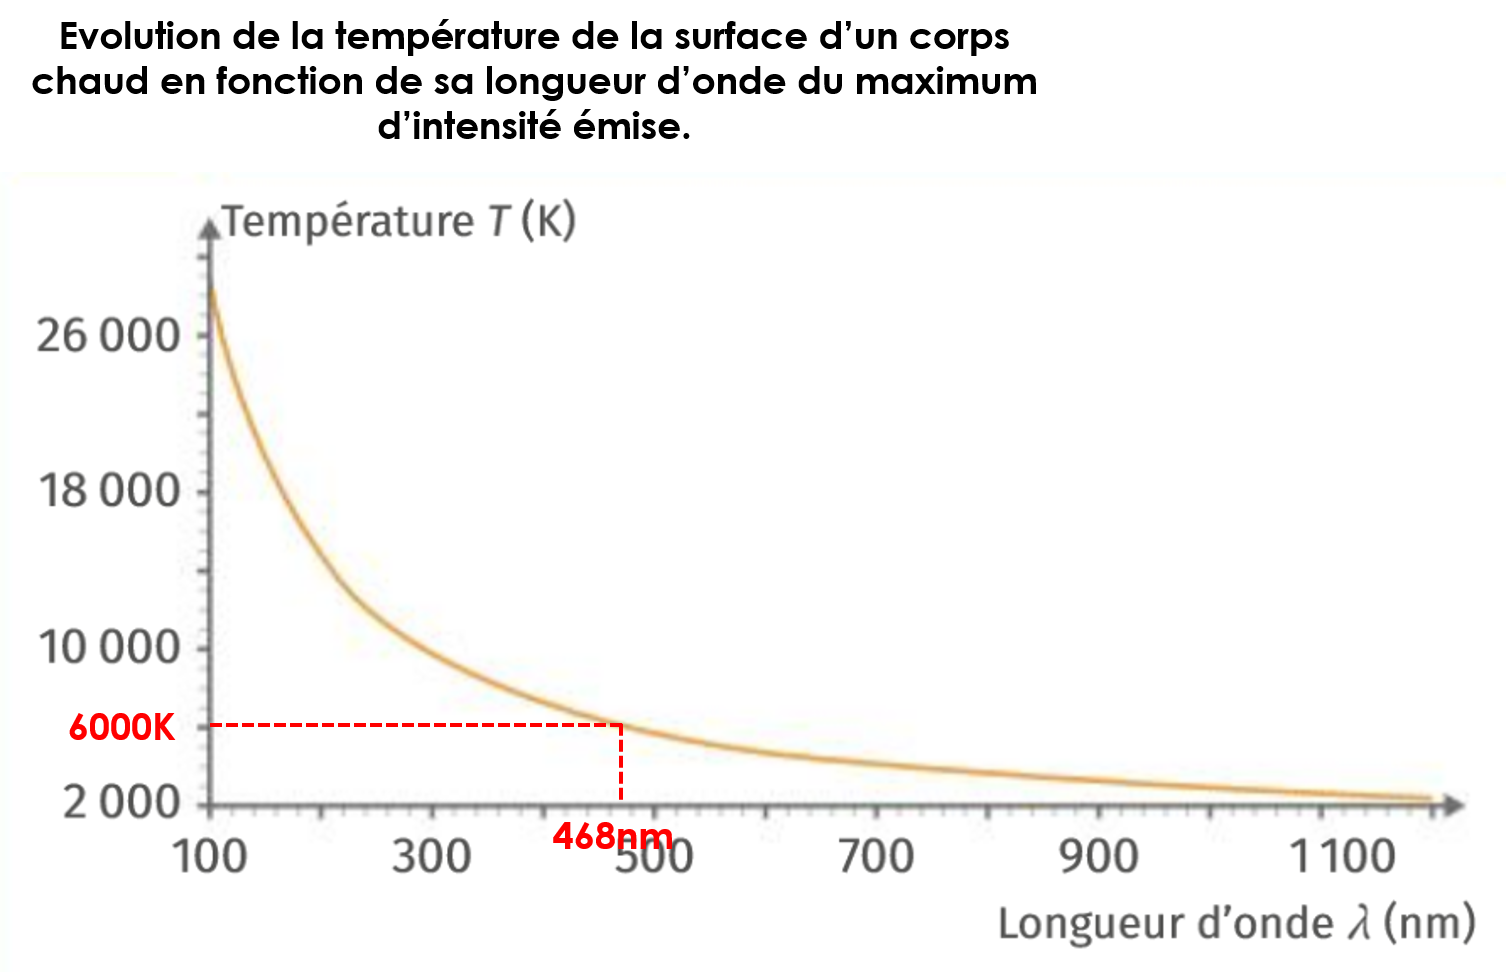
\includegraphics[scale=0.5]{Images/Correction_TemperatureEtoilePolaire.png}
\end{center}}{0}

\question{Conclure en justifiant si l'étoile Polaire fait partie des étoiles les plus chaudes de l'Univers.}{Non car les étoiles les plus chaudes ont une température de surface qui peut atteindre une température de 30 000~K d'après le document 3.}{0}

\subsection{Production par une espèce chimique}
\textcolor{blue}{Expérience :} On réalise le spectre de la lumière émise par une lampe à vapeur de mercure.\\
\textit{Observations :} \texteTrouMultiLignes{On observe un spectre d'émission discret en longueur d'onde qui est caractéristique de l'espèce chimique.}{2}


\begin{difficile}{\large Bilan sur la production de lumière}
\begin{flushleft}
    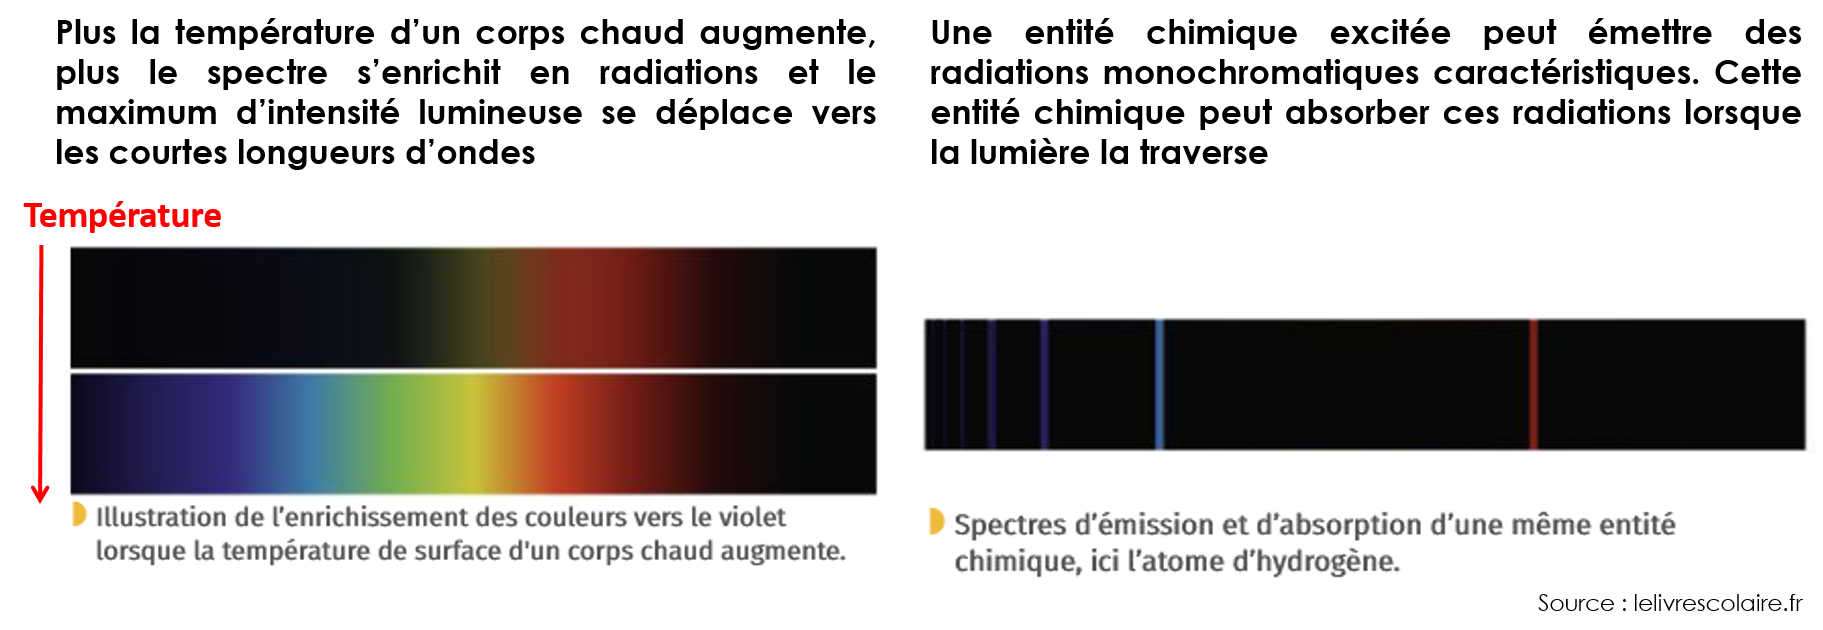
\includegraphics[scale=0.57]{Images/Bilan_productionlumiere.PNG}
    %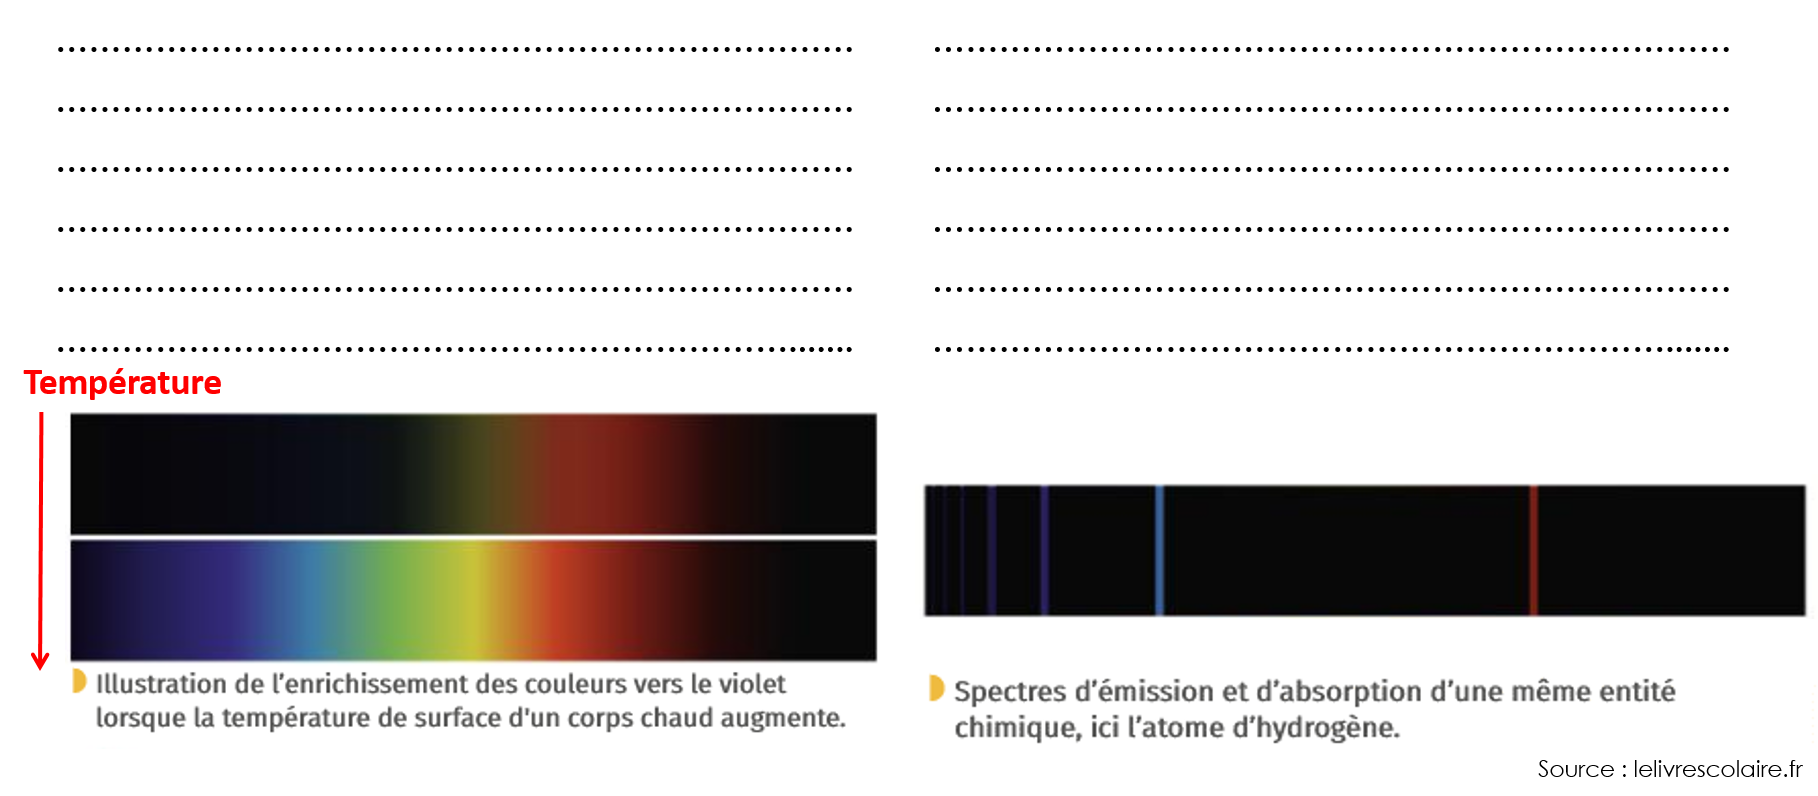
\includegraphics[scale=0.57]{Images/Bilan_productionlumiere_acompleter.png}
\end{flushleft}


\end{difficile}